\subsection{Terbium 155 Production}
% 155 Tb
Isotopes of Terbium, specifically the Terbium radioisotope quadruplet \cite{muller2012unique}, are highly regarded as a candidate for theranostic use where the four clinically useful candidates are: $^{149}\mathrm{Tb}$, $^{152}\mathrm{Tb}$, $^{155}\mathrm{Tb}$ and $^{161}\mathrm{Tb}$. The lowest mass isotope $^{149}\mathrm{Tb}$ ($T_{1/2} = 4.12$~\si{\hour}) decays via $\alpha$ emission, which could have many applications in oncology \cite{muller2017alpha} including treatment of leukemia and lymphoma \cite{beyer2004targeted}. The highest mass isotope $^{161}\mathrm{Tb}$ ($T_{1/2} = 6.89$~\si{\day}) decays exclusively via a low-energy $\beta^{-}$ decay route producing Auger electrons \cite{muller2012unique}, which is being explored at the trial phase as a treatment for prostate cancer \cite{baum2021first,muller2019terbium} and may be advantageous over $^{177}\mathrm{Lu}$ ($T_{1/2} = $~\si{}) to which $^{161}\mathrm{Tb}$ has similar decay characteristics with the production of more Auger electrons \cite{lehenberger2011low,grunberg2014anti}. Both $^{152}\mathrm{Tb}$ and $^{155}\mathrm{Tb}$ are useful in imaging; $^{152}\mathrm{Tb}$ decays via $\beta^{+}$ decay and therefore is useful in PET imaging \cite{muller2012unique}, whereas $^{155}\mathrm{Tb}$ ($T_{1/2} = 5.32$~\si{\day}) decays exclusively by electron capture and could be used in SPECT imaging to provide tumour imaging without a high radiation dose burden to the patient \cite{muller2012unique}.

These isotopes are typically produced using spallation methods; $^{161}\mathrm{Tb}$ is produced using neutron spallation of highly enriched $^{160}\mathrm{Gd}$ targets \cite{lehenberger2011low} whereas the other three isotopes have all been produced via high energy ($E_{e} = 1.4$~\si{\giga\electronvolt}) proton spallation \cite{muller2012unique} at the CERN-MEDICIS facility \cite{dos2014cern} with isotope separation on-line (ISOL) at the ISOLDE \cite{catherall2017isolde} facility. Deutron spallation techniques have also been used for the production of $^{155}\mathrm{Tb}$ using 34~\si{\mega\electronvolt} deutrons from the ARRONAX cyclotron \cite{duchemin2016deuteron}. 

Spallation methods with ISOL are typically expensive and complex facilities \cite{duchemin2016deuteron}, with only a handful worldwide such as the SPES-ISOLPHARM experiment \cite{andrighetto2019isolpharm} and no existing dedicated production facilities based on this method. The spallation and ISOL method consequently focuses on isotopes that are difficult to produce via more conventional research reactor and cyclotron based approaches. Therefore, an opportunity exists to develop alternative methods to produce isotopes solely available at ISOL facilities without the cost and complexity of high energy spallation and isotope separation on-line. The photonuclear route could provide some of these isotopes with less complexity; here we present a case study for one such isotope -- $^{155}\mathrm{Tb}$.

Terbium 155 is useful in SPECT imaging via the electron capture decay
\begin{equation}
^{155}\mathrm{Tb}\left(T_{1/2} = 5.32~\mathrm{\si{\day}}\right)\xrightarrow[]{\left(\mathrm{EC}, \mathrm{100\%}\right)}{}^{155}\mathrm{Gd},
\label{eq:Tb155_decay}
\end{equation}
which produces $\gamma$-rays at 86.55~\si{\kilo\electronvolt} (32\%) and 105.3~\si{\kilo\electronvolt} (25\%)\cite{muller2012unique} which are useful for SPECT imaging. A possible photonuclear route to produce $^{155}\mathrm{Tb}$ is via a photoneutron reaction $\left(\gamma,n\right)$ and subsequent exclusive $\beta^{+}$ decay from $^{156}\mathrm{Dy}$
\begin{equation}
^{156}\mathrm{Dy}\xrightarrow[]{\left(\gamma,n\right)}{}^{155}\mathrm{Dy}\left(T_{1/2} = 9.92~\mathrm{\si{\hour}}\right)\xrightarrow[]{\left(\beta^{+},\mathrm{100\%}\right)}{}^{155}\mathrm{Tb}.    
\label{eq:155Tb_photonuclear_production}
\end{equation}
Production via this route (Eq.~\ref{eq:155Tb_photonuclear_production}) would require a monoisotopic target of $^{156}\mathrm{Dy}$, however 156 Dysprosium isotope has a particularly low abunance in natural Dysprosium (0.056\%) and therefore requires enrichment. Enrichment via electromagnetic isotope separators, such as Caultrons \cite{bell1987stable}, can provide $< 34\%$ pure $^{156}\mathrm{Dy}$ whilst commercially $^{156}\mathrm{Dy}$ is available at $< 20.7\%$ enrichment \cite{}. Improvement in enrichment may be possible using lasers with methods such as separation of isotopes by laser excitation (SILEX)\cite{} \textcolor{blue}{**SILEX explanation, some examples ETC**} Because enrichment is so low for commercially available target isotopes, unlike in the $^{153}\mathrm{Sm}$ case, we must account for photoneutron reactions from other isotopes of Dysprosium in the assesment of the cross section.

The $^{156}\mathrm{Dy}\left(\gamma,n\right){}^{155}\mathrm{Dy}$ photoneutron reaction has a small cross section ($\sigma_{\mathrm{reac}} = 144\pm 44$~\si{\milli\barn}) \cite{vagena2017photodisintegration}, measured as an average cross section across a wide range of energies using a Bremsstrahlung method driven by an electron linac and tungsten target. However, several competing reactions to the $^{156}\mathrm{Dy}\left(\gamma,n\right){}^{155}\mathrm{Dy}$ reaction exist such as \cite{renstrom2018verification,vagena2017photodisintegration}
\begin{align}
^{163}\mathrm{Dy}&\xrightarrow[]{\left(\gamma,n\right)}{}^{162}\mathrm{Dy}, \\
^{162}\mathrm{Dy}&\xrightarrow[]{\left(\gamma,n\right)}{}^{161}\mathrm{Dy}, \\
^{158}\mathrm{Dy}&\xrightarrow[]{\left(\gamma,n\right)}{}^{157}\mathrm{Dy}, \\
^{156}\mathrm{Dy}&\xrightarrow[]{\left(\gamma,n\right)}{}^{155}\mathrm{Dy},
\label{eq:155Tb_photonuclear_disruptors}    
\end{align}
where higher order ($\gamma,2n$ etc.) reactions and those involving protons or alpha particles have no known measurement \cite{zerkin2018experimental}.

The photoneutron reaction cross sections as a function of incident photon energy are shown in Fig.~\ref{fig:}
\begin{figure}[!h]
\centering
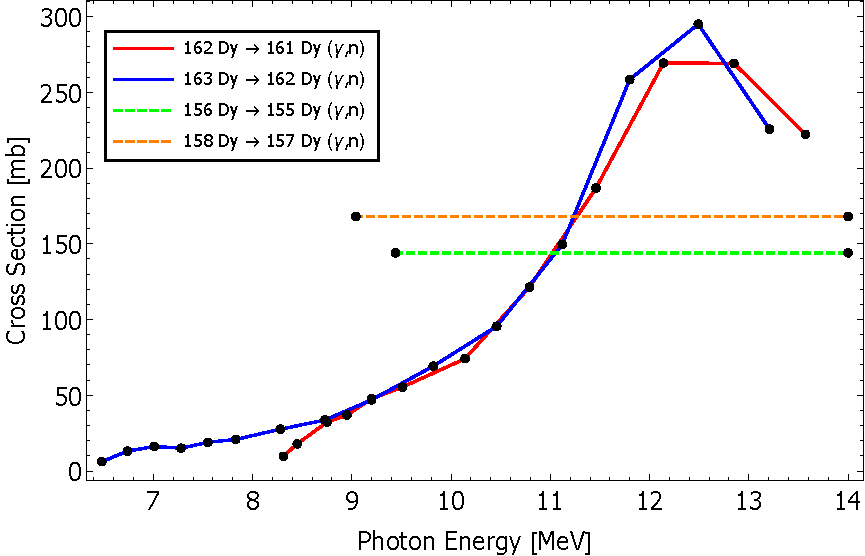
\includegraphics[width=0.8\textwidth]{Figures/DIANA_Inverse_Compton_Source_Design/DyLandscape.pdf}
\caption{Reaction cross section as a function of incident photon energy for measured photoneutron reactions from $^{\mathrm{nat}}\mathrm{Dy}$ including the desired $^{156}\mathrm{Dy}\left(\gamma,n\right){}^{155}\mathrm{Dy}$ (green \cite{vagena2017photodisintegration}) reaction and the disruptors $^{163}\mathrm{Dy}\left(\gamma,n\right){}^{162}\mathrm{Dy}$ (blue \cite{renstrom2018verification}), $^{162}\mathrm{Dy}\left(\gamma,n\right){}^{161}\mathrm{Dy}$ (red \cite{renstrom2018verification}) and $^{158}\mathrm{Dy}\left(\gamma,n\right){}^{157}\mathrm{Dy}$ (orange \cite{vagena2017photodisintegration}). Data for other $^{\mathrm{nat}}\mathrm{nat}$ reactions is unavailable. Dashed lines represent average cross section measurements \cite{vagena2017photodisintegration}, whereas full lines are cross section measurements made at varied incident photon energies. The EXFOR database has been used as a source of these measurements \cite{zerkin2018experimental}. }
\label{fig:Dy_cross_section_energy)}
\end{figure}

Fig.~\ref{fig:Dy_cross_section_energy)} shows that it will be difficult to produce no carrier added $^{155}\mathrm{Tb}$ from $^{\mathrm{nat}}\mathrm{Dy}$ as the competing reactions overlap in incident photon energy. Therefore, highly enriched dysprosium targets or chemical separation \cite{webster2019chemical}, which is also required in the spallation and ISOL approach, are necessary to production of high radioisotopic purity samples. The cross section measured by Vagena and Stoulos for the $^{156}\mathrm{Dy}\left(\gamma,n\right){}^{155}\mathrm{Dy}$ photoneutron reaction is $\sigma_{\mathrm{reac}} = 144\pm 44$~\si{\milli\barn}, which has a large error bar due to the nature of the Bremsstrahlung measurement method which has used integrated flux  within a large energy range defined by the reaction threshold and the maximum possible energy of the Bremsstrahlung source limited by the electron bunch energy of the linac. In contrast, precise measurements of the $^{162}\mathrm{Dy}\left(\gamma,n\right)$ and $^{163}\mathrm{Dy}\left(\gamma,n\right)$ reactions where narrower band photon spectra are used as the experimental probe \cite{renstrom2018verification}.

An order of magnitude estimate of the specific activity possible from  photoneutron production of $^{155}\mathrm{Dy}$ is possible using the collimated flux in a 0.5\% \textit{rms}  bandwidth of the DIANA ICS source, where we assume that the reaction cross section is constant at its peak value. This allows for an order of magnitude estimate of the specific activity of the $^{155}\mathrm{Tb}$ radioisotope which, as it has a longer half-life ($T_{1/2} = 5.32$~\si{\day}) than the intermediary $^{155}\mathrm{Dy}$ ($\left(T_{1/2} = 9.92\right)$~\si{\hour}), is the remaining isotope after a long irradiation. \textcolor{blue}{**THIS FEELS WOOLY, SURELY A MATHEMATICAL WAY TO DO THIS**} The measurement by Vagena and Stoulos \cite{vagena2017photodisintegration} is an average photoneutron reaction cross section within a photon energy range, therefore in order to correctly calculate the specific activity we make the assumption that the incident photon energy from DIANA, which we assume is steplessly variable, lies at the midpoint of this range $E_{\gamma} = 11.52$~\si{\mega\electronvolt}. Specific activity as a function of irradiation time is shown for the shorter-lived $^{155}\mathrm{Dy}$ intermediary in Fig.~\ref{fig:155Dy_specific_activity} with the 1$\sigma$ maximum and minimum cross section variation cases also plotted.
\begin{figure}[!h]
\centering
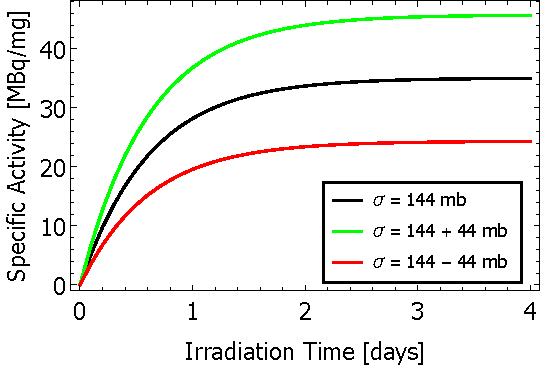
\includegraphics[width=0.6\textwidth]{Figures/DIANA_Inverse_Compton_Source_Design/155Dy_specific_activity.pdf}
\caption{Estimated specific activity of the produced $^{155}\mathrm{Dy}$ as a function of irradiation time using the collimated flux of the DIANA ICS source in a 0.5\% \textit{rms} bandwidth around a centroid scattered photon energy of $E_{\gamma} = 11.52$~\si{\mega\electronvolt}, the midpoint of the energy range measured by Vagena and Stoulos \cite{vagena2017photodisintegration} in the average reaction cross section measurement ($\sigma_{\mathrm{reac}} = 144$~\si{\milli\barn}) (black) and for values with $1\sigma$ error: $\sigma_{\mathrm{reac}} = 144 + 44$~\si{\milli\barn} (green) and $\sigma_{\mathrm{reac}} = 144 - 44$~\si{\milli\barn} (red).} 
\label{fig:155Dy_specific_activity}
\end{figure}
As shown in Fig.~\ref{fig:155Dy_specific_activity}, the specific activity of $^{155}\mathrm{Dy}$ saturates at $35.06\pm 10.71$~\si{\mega\becquerel}/\si{\milli\gram}, which occurs within a resonable $\sim$3 day duration. Assuming the same specific activity for the $^{155}\mathrm{Tb}$ radioisotope, the photoneutron production of $^{155}\mathrm{Tb}$ can be compared to spallation and ISOL methods via conversion of the specific activity to the widely used clinical units of
\si{\mega\becquerel}/\si{\nano\mole}. The CERN-MEDICIS facility have produced $^{155}\mathrm{Tb}$-cm09 at a specific activity of 0.64~\si{\mega\becquerel}/\si{\nano\mole} \cite{muller2012unique} whereas in the photoneutron production study here the specific activity is 5.43~\si{\kilo\becquerel}/\si{\nano\mole}, a factor of 117 below the spallation and ISOL method. However, the laser parameters in Table~\ref{tab:DIANA_laser_pulse_design_parameters} for the DIANA ICS source are conservative, the photonuetron production has not been optimised -- a standard 0.5\% \textit{rms} bandwidth collimated flux is used -- and the measurement of the cross section is just an average cross section, which is an underestimate as a narrowband $\gamma$-ray ICS source is capable of targeting resonance peaks. Hence, the estimated 5.43~\si{\kilo\becquerel}/\si{\nano\mole} specific activity of $^{155}\mathrm{Tb}$ shows promise for photonuclear production of $^{155}\mathrm{Tb}$.

In summary, production of $^{155}\mathrm{Tb}$ via the DIANA ICS source appears to be feasible and is a candiate for proof of principle medical isotope production using a DIANA ICS source. However, challenges to the photonuclear production of $^{155}\mathrm{Tb}$ exist, such as the enrichment of $^{156}\mathrm{Dy}$ targets and the requirement of improved measurement of the $^{156}\mathrm{Dy}\left(\gamma,n\right)$ cross section. At $\sim20$\% enrichment, $^{156}\mathrm{Dy}$ targets make production of no carrier added $^{155}\mathrm{Dy}$ difficult, though methods such as SILEX \cite{} may improve enrichment and chemical separation techniques \cite{webster2019chemical} can ameliorate this issue by removing impurities in the radioisotopic sample. The measurement of the $^{156}\mathrm{Dy}\left(\gamma,n\right)$ cross section is not fit for purpose, though it could be improved by measurement with ICS source, for example the higher quality measurements of $^{163}\mathrm{Dy}\left(\gamma,n\right)$ and $^{162}\mathrm{Dy}\left(\gamma,n\right)$ using the HI$\gamma$S ICS source \cite{renstrom2018verification}. Measuring photoneutron reaction cross sections could be a major application of the DIANA ICS source because DIANA can produce narrower band radiation than HI$\gamma$S, the leading $\gamma$-ray source, and also operates at a comparatively higher flux. These challenges are additional to the flux limitations and that are explored for the $^{153}\mathrm{Sm}$ photonuclear production case, therefore production of $^{155}\mathrm{Tb}$ is more complex.  
